\documentclass[9pt]{beamer}
\mode<presentation>

% ============================================================
% GENESIS IDEATHON: FINAL PRESENTATION TEMPLATE
% Edit the team details and the content inside each slide.
% Keep the setup section unchanged unless you want to customise
% the visual style of the presentation.
% ============================================================

% -------------------- THEME AND COLOURS ---------------------
\usetheme{Madrid}
\usecolortheme{default}
\usefonttheme{structurebold}
\setbeamercovered{invisible}
\setbeamertemplate{navigation symbols}{}

% Genesis green palette
\definecolor{GenesisGreen}{RGB}{35,105,70}
\definecolor{GenesisDarkGreen}{RGB}{22,75,51}
\definecolor{GenesisLightGreen}{RGB}{225,241,231}
\definecolor{GenesisCream}{RGB}{250,248,240}

% Apply the Genesis palette to Beamer elements
\setbeamercolor{structure}{fg=GenesisGreen}
\setbeamercolor{palette primary}{bg=GenesisDarkGreen,fg=white}
\setbeamercolor{palette secondary}{bg=GenesisGreen,fg=white}
\setbeamercolor{palette tertiary}{bg=GenesisDarkGreen,fg=white}
\setbeamercolor{palette quaternary}{bg=GenesisGreen,fg=white}
\setbeamercolor{frametitle}{bg=GenesisLightGreen,fg=GenesisDarkGreen}
\setbeamercolor{title}{fg=GenesisDarkGreen}
\setbeamercolor{block title}{bg=GenesisGreen,fg=white}
\setbeamercolor{block body}{bg=GenesisLightGreen,fg=black}
\setbeamercolor{item}{fg=GenesisGreen}
\setbeamercolor{section in toc}{fg=GenesisDarkGreen}
\setbeamercolor{subsection in toc}{fg=GenesisGreen}
\setbeamercolor{normal text}{fg=black,bg=white}
\setbeamercolor{author in head/foot}{bg=GenesisLightGreen,fg=GenesisDarkGreen}
\setbeamercolor{date in head/foot}{bg=GenesisLightGreen,fg=GenesisDarkGreen}

% ------------------------- PACKAGES -------------------------
\usepackage{graphicx}
\usepackage{amsfonts}
\usepackage{amsmath}
\usepackage{amssymb}
\usepackage{amsthm}
\usepackage{mathtools}
\usepackage{hyperref}
\usepackage[utf8]{inputenc}
\usepackage[T1]{fontenc}
\usepackage{lmodern}
\usepackage{tikz}
\usepackage[absolute,overlay]{textpos}
\usepackage{array}
\usepackage{colortbl}

% ---------------------- LAYOUT TUNING -----------------------
% Shared left/right margin: slide text, frame titles, and the
% footer all line up on the same vertical edge.
\newlength{\GenesisMargin}
\setlength{\GenesisMargin}{0.9cm}
\setbeamersize{text margin left=\GenesisMargin,text margin right=\GenesisMargin}

% Comfortable line and paragraph spacing
\linespread{1.12}
\setlength{\parskip}{0pt}

% Bullets: clean markers and more space between items
\setbeamertemplate{itemize item}[square]
\setbeamertemplate{itemize subitem}[circle]
\setbeamerfont{itemize/enumerate body}{size=\normalsize}
\setlength{\leftmargini}{1.4em}
\makeatletter
\def\@listi{\leftmargin\leftmargini
  \topsep 6pt plus 2pt minus 2pt
  \parsep 0pt
  \itemsep 10pt plus 3pt minus 3pt}
\let\@listI\@listi
\makeatother

% Rounded blocks (used for highlighted content)
\setbeamertemplate{blocks}[rounded][shadow=false]
\setbeamerfont{block title}{size=\normalsize,series=\bfseries}

% Frame title: fixed-height band with an accent rule, so the
% corner logo sits centred inside it on every content slide.
\setbeamerfont{frametitle}{size=\Large,series=\bfseries}
\setbeamertemplate{frametitle}{%
  \nointerlineskip
  \begin{beamercolorbox}[wd=\paperwidth,ht=0.58cm,dp=0.3cm,leftskip=\GenesisMargin]{frametitle}%
    \usebeamerfont{frametitle}\insertframetitle
  \end{beamercolorbox}%
  \nointerlineskip
  \begin{beamercolorbox}[wd=\paperwidth,ht=1.4pt,dp=0pt]{palette secondary}\end{beamercolorbox}%
}

% Numbered entries in the outline
\setbeamertemplate{section in toc}[sections numbered]
\setbeamerfont{section in toc}{size=\normalsize,series=\mdseries}

% --------------------- TEAM INFORMATION ---------------------
% Update these two commands. They appear in the footer of content slides.
\newcommand{\TeamNumber}{GEN26-A0H-I045}
\newcommand{\TeamName}{Sneakers}

% ------------------------- FOOTER ---------------------------
% Team number and team name appear at the bottom-left.
% The presentation date appears at the bottom-right.
\setbeamertemplate{footline}{%
  \leavevmode%
  \hbox{%
    \begin{beamercolorbox}[wd=.72\paperwidth,ht=3.0ex,dp=1.3ex,leftskip=\GenesisMargin]{author in head/foot}%
      \usebeamerfont{author in head/foot}\TeamNumber\ \textbar\ \TeamName
    \end{beamercolorbox}%
    \begin{beamercolorbox}[wd=.28\paperwidth,ht=3.0ex,dp=1.3ex,rightskip=\GenesisMargin]{date in head/foot}%
      \usebeamerfont{date in head/foot}\hfill\insertdate
    \end{beamercolorbox}%
  }%
}

% ---------------- PRESENTATION DETAILS ---------------------
% Replace these values with your team's actual information.
\title[farmX]{farmX: Smart Farming App}
\author{Team ID: \textit{GEN26-A0H-I045}\\[0.2cm]
Team Name: \textit{Sneakers}\\[0.2cm]
Domain 5: \textit{Food Security, Agriculture \& Rural Transformation}}
\institute{Amrita Vishwa Vidyapeetham, Coimbatore Campus}
\date{11th October 2026}

% -------------------------- LOGOS --------------------------
% The title slide displays all three logos.
% These filenames match the files shown in your Overleaf project.
% Each logo is vertically centred on the same line.
% Usage: \GenesisTitleLogo[height]{file}  (default height 1.35cm)
\newcommand{\GenesisTitleLogo}[2][1.35cm]{%
  \raisebox{-0.5\height}{\includegraphics[height=#1]{#2}}}
\titlegraphic{%
  \GenesisTitleLogo{Amrita_Vishwa_Vidyapeetham_Logo.png}%
  \hspace{0.7cm}%
  \GenesisTitleLogo[1.0cm]{iic_logo.png}%
  \hspace{0.7cm}%
  \GenesisTitleLogo[1.0cm]{genesis-iic.png}%
}

% Genesis logo at the top-right of content slides only.
% The title slide and outline slide do not use this logo placement.
% It is right-aligned to the slide margin and centred in the title band.
\newcommand{\GenesisCornerLogo}{%
  \begin{textblock*}{3cm}(\dimexpr\paperwidth-3cm-\GenesisMargin\relax,0.12cm)
    \raggedleft\includegraphics[height=0.64cm]{genesis-iic.png}
  \end{textblock*}%
}

% Title page: logos on top, then the title and team details (no footer).
\setbeamertemplate{title page}{%
  % Accent band along the top edge
  \begin{textblock*}{\paperwidth}(0cm,0cm)
    \begin{beamercolorbox}[wd=\paperwidth,ht=0.16cm,dp=0pt]{palette primary}\end{beamercolorbox}
  \end{textblock*}%
  \begin{minipage}[t][0.9\textheight][t]{\textwidth}
    % ---- Logos ----
    \vspace*{0.45cm}
    \begin{center}
      \inserttitlegraphic
    \end{center}
    \vspace{0.1cm}
    {\color{GenesisLightGreen}\rule{\textwidth}{1.2pt}\par}
    % ---- Title ----
    \vspace{0.3cm}
    \raggedright
    {\color{GenesisGreen}\rule{0.22\textwidth}{2.5pt}\par}
    \vspace{0.25cm}
    {\usebeamerfont{title}\usebeamercolor[fg]{title}\LARGE\bfseries\inserttitle\par}
    % ---- Team details ----
    \vspace{0.4cm}
    
\begin{tikzpicture}
      \node[fill=GenesisLightGreen,rounded corners=4pt,inner sep=0.35cm,
            text width=\dimexpr\textwidth-0.7cm\relax,align=left,
            font=\large] (card) {\insertauthor};
      \fill[GenesisGreen,rounded corners=1.5pt]
        ([xshift=0pt]card.north west) rectangle ([xshift=3pt]card.south west);
    \end{tikzpicture}\par
    \vspace{0.45cm}
    {\normalsize{\color{GenesisDarkGreen}\insertinstitute}\hfill\textbf{Date:} \insertdate\par}
  \end{minipage}%
}

% ------------------------- TABLES ---------------------------
% Column types: C = centred, L = left-aligned (both vertically centred).
\newcolumntype{C}[1]{>{\centering\arraybackslash}m{#1}}
\newcolumntype{L}[1]{>{\raggedright\arraybackslash}m{#1}}
% Header row and alternating body rows in the Genesis palette.
\newcommand{\GenesisHeadRow}{\rowcolor{GenesisGreen}}
\newcommand{\GenesisHead}[1]{\textcolor{white}{\textbf{#1}}}
\newcommand{\GenesisRowA}{\rowcolor{GenesisLightGreen}}
\newcommand{\GenesisRowB}{\rowcolor{GenesisLightGreen!40}}
% Wrapper: white rules between cells and roomy rows.
\newenvironment{GenesisTable}[1]{%
  \begin{center}
  \renewcommand{\arraystretch}{1.9}%
  \setlength{\tabcolsep}{4pt}%
  \arrayrulecolor{white}\setlength{\arrayrulewidth}{1.2pt}%
  \begin{tabular}{#1}}{%
  \end{tabular}
  \end{center}}

% Highlight card for the Yukthi ID on the last slide.
\newcommand{\GenesisIDCard}[2]{%
  \begin{tikzpicture}
    \node[fill=white,draw=GenesisGreen,line width=1.2pt,rounded corners=6pt,
          minimum width=7.6cm,minimum height=2.3cm,align=center,
          text=GenesisDarkGreen,font=\Huge\bfseries] (id) {#2};
    \node[fill=GenesisGreen,text=white,rounded corners=4pt,
          inner xsep=0.45cm,inner ysep=0.14cm,font=\normalsize\bfseries]
          at (id.north) {#1};
  \end{tikzpicture}%
}

% Placeholder box for the architecture / use-case diagram.
\newcommand{\GenesisDiagramBox}[1]{%
  \begin{tikzpicture}
    \node[draw=GenesisGreen,dashed,line width=0.8pt,rounded corners=4pt,
          fill=GenesisLightGreen!45,text=GenesisDarkGreen,
          text width=0.86\textwidth,minimum height=2.9cm,align=center,
          inner sep=6pt]{#1};
  \end{tikzpicture}%
}

% ============================================================
% DOCUMENT START
% ============================================================
\begin{document}

% ------------------------- TITLE SLIDE ----------------------
% Three logos on top, then team ID, team name, and domain.
\begin{frame}[plain]
  \titlepage
\end{frame}

% ------------------------- OUTLINE --------------------------
% This extra slide is separate from the 12 required content slides.
% It intentionally has no Genesis corner logo and no footer.
% (The footer is switched off in the group around the frame.)
{
\setbeamertemplate{footline}{}
\begin{frame}{Presentation Outline}
  \begin{columns}[T,onlytextwidth]
    \begin{column}{0.48\textwidth}
      \tableofcontents[sections={1-6}]
    \end{column}
    \begin{column}{0.48\textwidth}
      \tableofcontents[sections={7-12}]
    \end{column}
  \end{columns}
\end{frame}
}

% ============================================================
% SLIDE 1: PROBLEM STATEMENT
% ============================================================
\section{Problem Statement}
\begin{frame}{Problem Statement}
  \GenesisCornerLogo
  \begin{beamercolorbox}[rounded=true,sep=0.35cm,wd=\dimexpr\textwidth-0.7cm\relax]{block body}
    Small and medium-scale farmers need accessible support to identify crop disease,
    plan irrigation, sell produce and protect their fields. Scattered information
    and language barriers make these decisions harder.\par\vspace{0.25cm}
    \textbf{farmX brings crop care, weather, water planning, trade and field monitoring
    into one app, with help in the farmer's local language.}
  \end{beamercolorbox}
\end{frame}

% ============================================================
% SLIDE 2: PROBLEM UNDERSTANDING
% ============================================================
\section{Problem Understanding}
\begin{frame}{Problem Understanding}
  \GenesisCornerLogo
  \begin{itemize}
    \item \textbf{Who:} Small and medium-scale farmers who need timely, understandable
      advice and access to nearby and distant buyers.
    \item \textbf{Why:} Uncertain crop symptoms, changing weather, limited irrigation
      guidance, delivery barriers and difficulty using unfamiliar apps.
    \item \textbf{Consequences:} Delayed crop care, avoidable water use, difficult
      selling decisions and animal intrusion. Electric fences can also endanger animals.
  \end{itemize}
\end{frame}

% ============================================================
% SLIDE 3: EXISTING GAPS & CHALLENGES
% ============================================================
\section{Existing Gaps \& Challenges}
\begin{frame}{Existing Gaps \& Challenges}
  \GenesisCornerLogo
  \begin{itemize}
    \item \textbf{Disconnected decisions:} Crop diagnosis, weather, irrigation,
      selling and field monitoring need to work together in the farmer's daily routine.
    \item \textbf{Accuracy in real fields:} Forecasts need local evaluation. Disease
      photos vary with lighting and background, and broader pest recognition needs training.
    \item \textbf{Access and adoption:} Local-language support, reliable connectivity,
      affordable CCTV and dependable produce delivery are essential.
  \end{itemize}
\end{frame}

% ============================================================
% SLIDE 4: OUR PROPOSED SOLUTION
% ============================================================
\section{Our Proposed Solution}
\begin{frame}{Our Proposed Solution}
  \GenesisCornerLogo
  \begin{itemize}
    \setlength{\itemsep}{5pt}
    \item \textbf{Weather report:} Combine The Weather Company, AccuWeather and
      Foreca forecasts, aiming for more reliable local guidance.
    \item \textbf{Crop Doctor:} Use ConvTransNet-S for leaf disease symptoms,
      with further training planned for insect and pest damage.
    \item \textbf{Irrigation calculator:} Use field dimensions, crop, sowing season,
      soil and app weather to estimate water required in litres.
    \item \textbf{Online market:} Sell to nearby and long-distance buyers,
      with delivery through a contracted transport service.
    \item \textbf{Field monitoring:} Live CCTV, an animal-intrusion alarm and farmer
      alerts support crop protection and reduce reliance on electric fences.
    \item \textbf{AI assistant:} Answer queries and teach app use in the local
      language through voice chat and typed chat.
  \end{itemize}
\end{frame}

% ============================================================
% SLIDE 5: TECHNICAL APPROACH
% ============================================================
\section{Technical Approach}
\begin{frame}{Technical Approach}
  \GenesisCornerLogo
  \begin{center}
    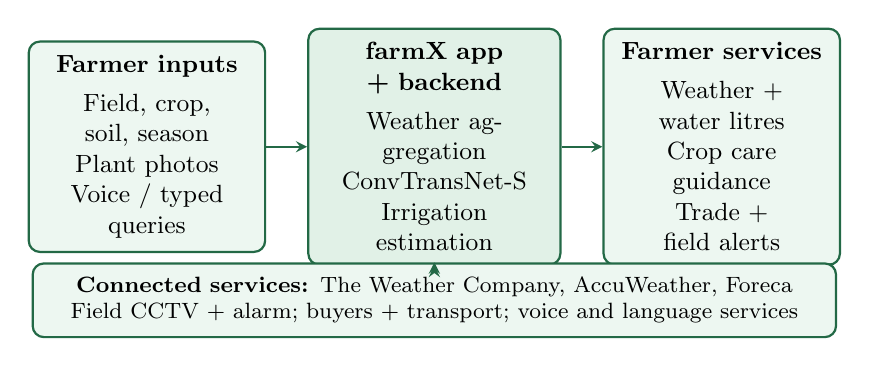
\begin{tikzpicture}[>=stealth,
      farmnode/.style={draw=GenesisGreen,line width=0.8pt,rounded corners=4pt,
        fill=GenesisLightGreen!60,align=center,font=\small,
        inner sep=5pt,minimum height=2.1cm}]
      \node[farmnode,text width=2.65cm] (input) at (-3.65,0)
        {\textbf{Farmer inputs}\\[3pt]Field, crop, soil, season\\Plant photos\\Voice / typed queries};
      \node[farmnode,text width=2.85cm,fill=GenesisLightGreen] (core) at (0,0)
        {\textbf{farmX app + backend}\\[3pt]Weather aggregation\\ConvTransNet-S\\Irrigation estimation};
      \node[farmnode,text width=2.65cm] (output) at (3.65,0)
        {\textbf{Farmer services}\\[3pt]Weather + water litres\\Crop care guidance\\Trade + field alerts};
      \draw[->,thick,GenesisGreen] (input.east) -- (core.west);
      \draw[->,thick,GenesisGreen] (core.east) -- (output.west);
      \node[farmnode,text width=9.85cm,minimum height=0.8cm,font=\footnotesize]
        (services) at (0,-1.95)
        {\textbf{Connected services:} The Weather Company, AccuWeather, Foreca\\
         Field CCTV + alarm; buyers + transport; voice and language services};
      \draw[<->,thick,GenesisGreen] (core.south) -- (services.north);
    \end{tikzpicture}
  \end{center}
  \vspace{-0.1cm}
  \begin{center}
    \small Weather updates feed the irrigation estimate.
    Animal detection triggers a field alarm and an app alert.
  \end{center}
  \begin{beamercolorbox}[rounded=true,sep=0.22cm,wd=\dimexpr\textwidth-0.44cm\relax]{block body}
    \small\textbf{Proposed Tech Stack}\par\vspace{0.08cm}
    \begin{tabular}{@{}p{0.41\textwidth}p{0.47\textwidth}@{}}
      \textbf{Frontend:} Flutter & \textbf{Database:} PostgreSQL \\[0.07cm]
      \textbf{Backend:} Python / FastAPI & \textbf{AI / APIs:} ConvTransNet-S, weather, voice \\
    \end{tabular}
  \end{beamercolorbox}
\end{frame}

% ============================================================
% SLIDE 6: INNOVATION & UNIQUENESS
% ============================================================
\section{Innovation \& Uniqueness}
\begin{frame}{Innovation \& Uniqueness}
  \GenesisCornerLogo
  \begin{itemize}
    \item \textbf{What is new or different?} farmX combines crop diagnosis,
      weather, irrigation estimates, produce sales, field monitoring and AI help
      in one app.
    \item \textbf{Why does this approach suit farmers?} Watering estimates use
      the farmer's field, crop, soil, season and weather. Local-language voice
      and text make guidance easier to use.
    \item \textbf{What is the key differentiator?} Weather updates also inform
      irrigation, produce sales include partner delivery, and animal detection
      triggers alarms and farmer alerts to reduce reliance on electric fences.
  \end{itemize}
\end{frame}

% ============================================================
% SLIDE 7: FEASIBILITY & SCALABILITY
% ============================================================
\section{Feasibility \& Scalability}
\begin{frame}{Feasibility \& Scalability}
  \GenesisCornerLogo
  \begin{itemize}
    \item \textbf{Feasibility:} Begin with Crop Doctor, weather, irrigation and
      the voice/text assistant. Pilot with farmers, then integrate CCTV, alarms,
      the marketplace and transport operations.
    \item \textbf{Scalability:} Reuse the backend across crops and regions.
      Add validated disease classes, local languages and delivery partners in stages.
    \item \textbf{Risks and checks:} Validate field diagnosis, insect/pest training,
      forecast accuracy and animal alerts. Plan for API licences, connectivity,
      hardware upkeep and transport costs.
  \end{itemize}
\end{frame}

% ============================================================
% SLIDE 8: COST FOR PRODUCT
% ============================================================
\section{Cost for Product}
\begin{frame}{Cost for Product (Optional)}
  \GenesisCornerLogo
  \begin{itemize}
    \setlength{\itemsep}{7pt}
    \item \textbf{Build:} Student development using existing laptops and open-source
      tools. Budget separately for app integration and field testing.
    \item \textbf{Operate:} Recurring cloud hosting, AI inference, database,
      weather-data licences and voice services. Fees depend on pilot usage.
    \item \textbf{Field kit:} CCTV camera, alarm, power and connectivity per field.
      Final cost requires provider quotations and the number of pilot farms.
  \end{itemize}
  \vspace{0.18cm}
  \begin{beamercolorbox}[rounded=true,sep=0.25cm,wd=\dimexpr\textwidth-0.5cm\relax]{block body}
    \textbf{Revenue model:} 20\% of each sale: 10\% for contracted transport
    and 10\% for farmX.\par\vspace{0.08cm}
    \small On a Rs.~1,000 sale: farmer Rs.~800, transport Rs.~100, farmX Rs.~100.
  \end{beamercolorbox}
  \vspace{0.1cm}
  {\scriptsize Planning model. Total launch budget awaits quotations and pilot scope.}
\end{frame}

% ============================================================
% SLIDE 9: USE CASES
% ============================================================
\section{Use Cases}
\begin{frame}{Use Cases}
  \GenesisCornerLogo
  \begin{itemize}
    \item \textbf{1. Spot crop disease:} A farmer uploads a leaf photo to Crop Doctor
      and hears the result and guidance in the local language. Voice or typed queries
      provide further help.
    \item \textbf{2. Plan watering:} A farmer enters field dimensions, crop,
      sowing season and soil. The app combines these with its weather report to
      estimate water required in litres and avoid unnecessary watering.
    \item \textbf{3. Sell and monitor remotely:} A farmer sells produce to a local
      or distant buyer with partner delivery. Live field CCTV also sends an animal
      intrusion alert while the field alarm sounds.
  \end{itemize}
\end{frame}

% ============================================================
% SLIDE 10: IMPACTS AND BENEFITS
% ============================================================
\section{Impacts and Benefits}
\begin{frame}{Impacts and Benefits}
  \GenesisCornerLogo
  \begin{itemize}
    \item \textbf{For farmers:} Earlier crop-care decisions, clearer watering
      guidance, access to buyers and delivery, and app help through local-language
      voice and typed chat.
    \item \textbf{For farms and animals:} Aim to reduce avoidable water use,
      support crop health and reduce animal deaths from electric fences by using
      intrusion alarms and farmer alerts.
    \item \textbf{Measure in the pilot:} Field diagnosis accuracy, forecast error,
      water used, completed sales, farmer usability and animal-alert false alarms.
      These benefits require field validation.
  \end{itemize}
\end{frame}

% ============================================================
% SLIDE 11: SUSTAINABLE DEVELOPMENT GOALS
% ============================================================
\section{Sustainable Development Goals}
\begin{frame}{Sustainable Development Goals (SDGs)}
  \GenesisCornerLogo
  \begin{GenesisTable}{C{2.1cm}|C{2.25cm}|L{2.45cm}|L{2.95cm}}
    \GenesisHeadRow
    \GenesisHead{SDG Number} & \GenesisHead{Target Number} & \GenesisHead{Goal Name} & \GenesisHead{Connection} \\ \hline
    \GenesisRowA
    \textbf{SDG~2} & Target 2.4 & Zero Hunger & Crop care and weather guidance support resilient, sustainable farming. \\ \hline
    \GenesisRowB
    \textbf{SDG~6} & Target 6.4 & Clean Water and Sanitation & Weather-aware irrigation estimates support efficient water use. \\
  \end{GenesisTable}
  \vspace{0.12cm}
  {\scriptsize Intended contributions. Sources:
    \href{https://sdgs.un.org/goals/goal2}{UN SDG 2, Target 2.4};
    \href{https://sdgs.un.org/goals/goal6}{UN SDG 6, Target 6.4}.}
\end{frame}

% ============================================================
% SLIDE 12: INDIVIDUAL MEMBER CONTRIBUTION
% ============================================================
\section{Individual Member Contribution}
\begin{frame}{Individual Member Contribution}
  \GenesisCornerLogo
  \begin{GenesisTable}{C{2.6cm}|L{7.0cm}}
    \GenesisHeadRow
    \GenesisHead{Member} & \GenesisHead{Contribution or responsibility} \\ \hline
    \GenesisRowA
    \textbf{S. Kaveen} & \textbf{Team Leader:} Team coordination, research, app design, testing and presentation. \\ \hline
    \GenesisRowB
    \textbf{Alen Jomon} & Weather report and irrigation calculator. \\ \hline
    \GenesisRowA
    \textbf{Abijith raja S} & Crop Doctor and AI assistant. \\ \hline
    \GenesisRowB
    \textbf{Iniyan J} & Online market, delivery and CCTV alerts. \\
  \end{GenesisTable}
\end{frame}

% ============================================================
% LAST SLIDE: YUKTI ID
% This closing slide is not listed in the outline.
% ============================================================
\begin{frame}{Yukti ID}
  \GenesisCornerLogo
  % Replace "[Enter Yukthi ID]" with your team's Yukthi ID.
  \begin{center}
    \GenesisIDCard{Yukti ID}{[IR2026-1051040]}
  \end{center}
\end{frame}

\end{document}
